\documentclass[a4paper, 11pt]{article}
\usepackage{comment}
\usepackage{fullpage}
\usepackage{amsmath}
\usepackage{amssymb}
\usepackage{amsthm}
\usepackage{mathtools}
\usepackage{siunitx}
\usepackage{xfrac}
\usepackage{icomma}
\usepackage[section,below]{placeins}
\usepackage[labelfont=bf,font=small,width=0.9\textwidth]{caption}
\usepackage{subcaption}
\usepackage{graphicx}
\usepackage{grffile}
\usepackage{float}
\floatplacement{figure}{htbp}
\floatplacement{table}{htbp}
\usepackage{booktabs}
\usepackage{hyperref}
\usepackage{pdfpages}
\usepackage{cite}
\sisetup{separate-uncertainty=true}

\begin{document}
\newtheorem{lemma}{Lemma}
\noindent
\centerline{\small{\textsc{Michigan State University}}} \\
\large{\textbf{CMSE 823 – Numerical Linear Algebra \hfill Spring 2020 \\
Final Exam} \\
Alexander Harnisch \\}
\noindent\makebox[\linewidth]{\rule{\textwidth}{0.4pt}}

\section*{Problem 1}
\subsection*{(a)}
For $A \in \mathbb{C}^{m\times n}$:
\begin{equation}
  \Vert A\Vert_\infty \leq \sqrt{n}\Vert A \Vert_2.
  \label{eqn:a}
\end{equation}

\begin{proof}
First, using the definition~\cite[(3.2)]{tb} of the 2-norm and infinity norm
for any $x \in \mathbb{C}^n$:
\begin{equation*}
  \Vert x \Vert_2^2 = \sum_{i = 1}^n x_i^2 \leq n \max_{1 \leq i \leq m} x_i^2 = n \Vert x\Vert_\infty^2.
\end{equation*}
And thus
\begin{equation}
  \Vert x \Vert_2 \leq \sqrt{n} \Vert x \Vert_\infty \Leftrightarrow
  \frac{1}{\Vert x \Vert_\infty} \leq \frac{\sqrt{n}}{\Vert x \Vert_2},\quad x \neq 0.
  \label{1}
\end{equation}
Additionally, we have
\begin{equation}
  \Vert x \Vert_\infty = \max_{1 \leq i \leq n} \vert x_i \vert \leq
  \sqrt{\sum_{i=1}^n x_i^2} = \Vert x\Vert_2 \Leftrightarrow \frac{1}{\Vert
  x\Vert_2} \leq \frac{1}{\Vert x\Vert_\infty}, \quad x \neq 0.
  \label{2}
\end{equation}
Combining these results with the definition of the induced matrix
norm~\cite[(3.6)]{tb}, we find the inequality:
\begin{equation*}
  \Vert A \Vert_\infty = \sup_{x \in \mathbb{C}^n,\,x \neq 0} \frac{\Vert Ax
  \Vert_\infty}{\Vert x \Vert_\infty} \stackrel{\eqref{2}}{\leq}
  \sup_{x \in \mathbb{C}^n,\,x \neq 0} \frac{\Vert Ax \Vert_2}{\Vert x
  \Vert_\infty}
  \stackrel{\eqref{1}}{\leq}
  \sup_{x \in \mathbb{C}^n,\,x \neq 0} \frac{\sqrt{n}\Vert Ax \Vert_2}{\Vert x
  \Vert_2} = \sqrt{n} \Vert A \Vert_\infty
\end{equation*}
\end{proof}

We also find the inequality
\begin{equation*}
  \Vert A \Vert_2 \leq \sqrt{m} \Vert A \Vert_\infty.
\end{equation*}
\begin{proof}
\begin{equation*}
  \Vert A \Vert_2 = \sup_{x \in \mathbb{C}^n,\,x \neq 0} \frac{\Vert Ax
  \Vert_2}{\Vert x \Vert_2} \stackrel{\eqref{1}}{\leq}
  \sup_{x \in \mathbb{C}^n,\,x \neq 0} \frac{\sqrt{m}\Vert Ax \Vert_\infty}{\Vert x
  \Vert_2}
  \stackrel{\eqref{2}}{\leq}
  \sup_{x \in \mathbb{C}^n,\,x \neq 0} \frac{\sqrt{m}\Vert Ax \Vert_\infty}{\Vert x
  \Vert_\infty} = \sqrt{m} \Vert A \Vert_\infty
\end{equation*}
\end{proof}

\subsection*{(b)}
The inequality~\eqref{eqn:a} is sharp.
\begin{proof}
  To show that the inequality is sharp, we only need to find an example for which equality holds. Such an example is:
  \begin{equation*}
    M =
    \begin{bmatrix}
    1 & 1 \\
    0 & 0 \\
    \end{bmatrix}.
  \end{equation*}
  $\Vert M \Vert_\infty = 2$ and $\Vert M \Vert_2 = \sqrt{2}$ so
  \begin{equation*}
    \Vert M \Vert_\infty = \sqrt{2} \Vert M \Vert_2.
  \end{equation*}
\end{proof}

\section*{Problem 2}
Let $A \in \mathbb{C}^{m \times n}$ with $m \geq  n$. $A^{*}A$ is non-singular
if and only if $A$ has full rank.
\begin{proof}
The rank of $A$ is the number of non-zero singular values~\cite[Theorem
5.1]{tb}.  Let the SVD of $A$ be $A = U\Sigma V^*$. Then it follows, that $A$
is of full rank if and only if $\Sigma$ is of full rank and
\begin{equation*}
  A^*A = V \Sigma^* U^* U \Sigma V^* = V \Sigma^* \Sigma V^* = V \Sigma^2 V^*.
\end{equation*}
This is an eigenvalue decomposition (similarity transformation). Therefore,
$A^*A$ is of full rank if and only if $\Sigma^2$ is of full rank, which is of
full rank if and only if $\Sigma$ is of full rank. $\Sigma$ is diagonal and its
diagonal entries are the singular values of $A$,  so $\Sigma$ is of full rank
if and only if $A$ is of full rank. $A^*A$ is a square matrix, so it is
non-singular if and only if it has full rank. We conclude that $A^*A$ is
non-singular if and only if $A$ is of full rank.
\end{proof}

\section*{Problem 3}
Let $A \in \mathbb{C}^{m \times m}$, and let $a_j$ be its $j$-th column. Then:
\begin{equation}
  \vert \det(A) \vert \leq \prod_{j = 1}^m \Vert a_j\Vert_2.
  \label{3_1}
\end{equation}
\begin{proof}
  Let $A = QR$ be the QR decomposition of $A$. Let $q_j$ be the $j$-th
  column of $Q$ and $r_{ij}$ be the ($i$, $j$) entry of $R$.

  From $a_j = \sum_{i=1}^j r_{ij}q_i$~\cite[(7.3)]{tb}
  and $r_{ij} = q_i^*a_j$ for $i \neq j$~\cite[(7.7)]{tb} and the fact that the
  columns of $Q$ are orthonormal, it follows directly, that:
  \begin{equation}
  \Vert a_j \Vert_2^2 = \left(\sum_{i=1}^j r_{ij}q_i\right)^2 = \sum_{i=1}^j
  r_{ij}^2 = \sum_{i=1}^j \vert q_i^* a_j\vert^2.\\ \label{3_lemma}
  \end{equation}

  With that, we find:
  \begin{align*}
    \det(A)^2 &= \det(A^*A) = \det(R^*Q^*QR) = \det(R^*R) = \det(R)^2 \\
    &= \prod_{j = 1}^m \vert r_{jj}\vert^2 \stackrel{\text{\cite[(7.7)]{tb}}}{=}
    \prod_{j = 1}^m \vert q_j^*a_j\vert^2 \\
    &\leq \prod_{j = 1}^m \sum_{i = 1}^j \vert q_i^*a_j\vert^2 \stackrel{\text{\eqref{3_lemma}}}{=} \prod_{j = 1}^m \Vert a_j\Vert_2^2
  \end{align*}
  Taking the square root gives \eqref{3_1}.
\end{proof}

\section*{Problem 4}
\subsection*{(a)}
The primary textbook does not mention an SVD theorem. It
does, however, give a formal definition of the Singular Value
decomposition~\cite[pp. 28-29]{tb}. The existence and uniqueness is stated and
proven~\cite[Theorem 4.1]{tb}. A slide titled ``SVD: Theorem'' can be found
in~\cite{slides}. It states, that
\begin{enumerate}
  \item Every matrix $A \in \mathbb{C}^{m\times n}$ has an SVD.
  \item The singular values $\{\sigma_i\}$ are uniquely determined.
  \item If $A \in \mathbb{C}^{m\times n}$ and the singular values $\sigma_i$ are distinct, then the left and right singular vectors $\{u_i\}$ and $\{v_i\}$ are uniquely determined up to complex signs (i.e. complex scalar factors of modulus 1).
\end{enumerate}
This is the same as Theorem 4.1 from~\cite{tb}.

\subsection*{(b)}
Let $A \in \mathbb{C}^{m\times n}$. Set $\sigma = \Vert A\Vert_2$. There are
vectors $v \in \mathbb{C}^{n}$ and $u \in \mathbb{C}^m$ with $\Vert v\Vert_2 =
\Vert u\Vert_2 = 1$ such that $Av=\sigma u$.
\begin{proof}
  Let $A = U\Sigma V^*$ be the SVD of $A$. $\Sigma$ is diagonal and its entries
  are the singular values of $A$. $\sigma = \Vert A\Vert_2$ is the largest
  singular value of $A$~\cite[Theorem 5.3]{tb}. Thus:
  \begin{equation}
    AV = U\Sigma \Rightarrow Av = \sigma u,
  \end{equation}
  where $v$ is the right and $u$ the left normalized singular vector
  corresponding to the largest singular value $\sigma$ of $A$.
\end{proof}
This proof might be circular, depending on how the SVD theorem stated above has
been proven. An alternative proof is the compactness argument of the induced 2
norm used in the proof of Theorem 4.1 in \cite{tb}. This proof is also
given in \cite{slides}:
\begin{figure}[H]
  \centering
  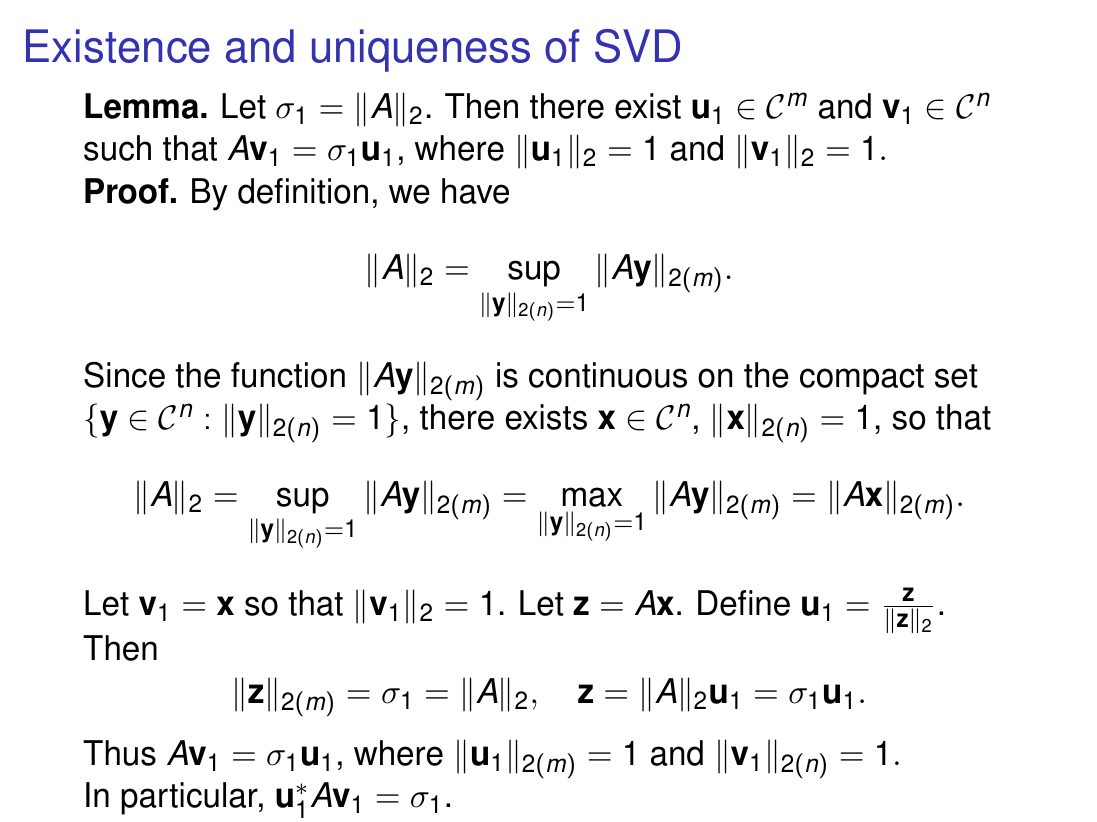
\includegraphics[width=\textwidth]{./compactness_slide.png}
  \caption{Proof of (b) given in \cite{slides}.}
\end{figure}

\subsection*{(c)}
A reduced SVD of
\begin{equation*}
 A =
  \begin{bmatrix}
  0 & 0 \\
  0 & 0 \\
  0 & 2 \\
  \end{bmatrix}
\end{equation*}
is
\begin{equation*}
 A = U\Sigma V^* =
  \begin{bmatrix}
  0 & 1 \\
  0 & 0 \\
  -1 & 0 \\
  \end{bmatrix}
  \begin{bmatrix}
  2 & 0 \\
  0 & 0 \\
  \end{bmatrix}
  \begin{bmatrix}
  0 & -1 \\
  1 & 0 \\
  \end{bmatrix}.
\end{equation*}
To make it a full SVD, we only need to make the columns of $U$ a full basis of
$\mathbb{R}^{3}$ by adding the column $(0, 1, 0)^{\top}$ and adding a row of zeros
to $\Sigma$.

Just as a short justification of the result: For this simple
matrix I could come up with it in my head by knowing that $\Sigma$ is a
diagonal matrix with the square roots of the eigenvalues of $A^\top A$
on its diagonal~\cite[Theorem 5.4]{tb}.

\section*{Problem 5}
We want to solve the least-squares problem $\min_{x \in \mathbb{R}^2} \Vert Ax
- b\Vert_2$, where $b
= (0, 0, 3, 2)^\top$ and
\begin{equation*}
  A =
  \begin{bmatrix}
  1 & -1 \\
  0 & 0 \\
  2 & 1 \\
  0 & 2 \\
  \end{bmatrix}
\end{equation*}
using Algorithm 11.2 defined in \cite{tb}. The result can be cross-checked
numerically and by using \cite[(11.12)]{tb}.

\textbf{1.} The first step is to compute the QR decomposition of $A$. This can
most conveniently be achieved by Gram-Schmidt Orthogonalization or Householder
Triangularization. Let's choose the former, because it requires less typing:
\begin{equation*}
  q_1' = a_1 =
  \begin{bmatrix}
  1  \\
  0 \\
  2 \\
  0 \\
  \end{bmatrix}
\end{equation*}
\begin{equation*}
  r_{1 1} = \Vert q_1'\Vert = \sqrt{1^2 + 2^2} = \sqrt{5}
\end{equation*}
\begin{equation*}
  q_1 = \frac{q_1'}{\Vert q_1'\Vert} = \frac{1}{\sqrt{5}}
  \begin{bmatrix}
  1  \\
  0 \\
  2 \\
  0 \\
  \end{bmatrix}
\end{equation*}
\begin{equation*}
  r_{1 2} = q_1^{\top}a_2 = \frac{1}{\sqrt{5}}(-1 + 2) = \frac{1}{\sqrt{5}}
\end{equation*}
\begin{equation*}
  q_2' = a_2 - r_{1 2}q_1 =
  \begin{bmatrix}
  -1  \\
  0 \\
  1 \\
  2 \\
  \end{bmatrix}
  - \frac{1}{5}
  \begin{bmatrix}
  1  \\
  0 \\
  2 \\
  0 \\
  \end{bmatrix}
  =
  \frac{1}{5}
  \begin{bmatrix}
  -6  \\
  0 \\
  3 \\
  10 \\
  \end{bmatrix}
\end{equation*}
\begin{equation*}
  r_{2 2} = \Vert q_2' \Vert = \sqrt{5.8}
\end{equation*}
\begin{equation*}
  q_2 = \frac{q_2'}{\Vert q_2'\Vert} = \frac{1}{5\sqrt{5.8}}
  \begin{bmatrix}
  -6  \\
  0 \\
  3 \\
  10 \\
  \end{bmatrix}
\end{equation*}
And thus:
\begin{equation*}
  A = QR =
  \begin{bmatrix}
  \frac{1}{\sqrt{5}} & -\frac{6}{5\sqrt{5.8}} \\
  0 & 0 \\
  \frac{2}{\sqrt{5}} & \frac{3}{5\sqrt{5.8}} \\
  0 & \frac{10}{5\sqrt{5.8}} \\
  \end{bmatrix}
  \begin{bmatrix}
  \sqrt{5} & \frac{1}{\sqrt{5}} \\
  0 & \sqrt{5.8} \\
  \end{bmatrix}.
\end{equation*}

\textbf{2.} Compute $y = Q^*b = Q^\top b$:
\begin{equation*}
  y^\top = b^\top Q =
  \begin{bmatrix}
    0 & 0 & 3 & 2
  \end{bmatrix}
  \begin{bmatrix}
  \frac{1}{\sqrt{5}} & -\frac{6}{5\sqrt{5.8}} \\
  0 & 0 \\
  \frac{2}{\sqrt{5}} & \frac{3}{5\sqrt{5.8}} \\
  0 & \frac{10}{5\sqrt{5.8}} \\
  \end{bmatrix}
  =
  \begin{bmatrix}
    \frac{6}{\sqrt{5}} & \frac{29}{5\sqrt{5.8}}
  \end{bmatrix}
\end{equation*}

\textbf{3.} Solve $Rx=y$ for $x$, which solves $\min_{x \in \mathbb{R}^2} \Vert
Ax - b\Vert_2$.
\begin{equation*}
  \begin{bmatrix}
  \sqrt{5} & \frac{1}{\sqrt{5}} \\
  0 & \sqrt{5.8} \\
  \end{bmatrix}
  \begin{bmatrix}
    x_1 \\
    x_2 \\
  \end{bmatrix}
  =
  \begin{bmatrix}
    \frac{6}{\sqrt{5}} \\
    \frac{29}{5\sqrt{5.8}}
  \end{bmatrix}
\end{equation*}

Note that $\sqrt{5.8} = \frac{\sqrt{145}}{5} = \frac{29}{5\sqrt{5.8}}$, thus
the solution is
\begin{equation*}
  x =
  \begin{bmatrix}
    1 \\
    1 \\
  \end{bmatrix}.
\end{equation*}.

\section*{Problem 6}
Let $A \in \mathbb{R}^{n \times n}$ be symmetric and positive definite with $n
= j + k$. Partition $A$ into the following 2 b 2 blocks:
\begin{equation*}
  A =
  \begin{bmatrix}
    A_{11} & A_{12} \\
    A_{21} & A_{22} \\
  \end{bmatrix}
\end{equation*}
where $A_{11}$ is $j \times j$ and $A_{22}$ is $k \times k$. Let $R_{11}$ be
the  Cholesky factor of $A_{11}$: $A_{11} =  R_{11}^\top R_{11}$, where
$R_{11}$ is upper-triangular with positive main-diagonal entries. Let $R_{12} =
(R_{11}^{-1})^\top A_{12}$ and let $\tilde{A}_{22} = A_{22} - R_{12}^\top
R_{12}$.

\subsection*{(a)}
$A_{11}$ is positive definite.
\begin{proof}
We know that $A$ is positive definite:
\begin{equation*}
  x^\top A x > 0 \quad \forall x \in \mathbb{R}^n \setminus \{0\}.
\end{equation*}
From that it follows, that for
\begin{equation*}
  \tilde{x} \in \left\{(y, 0)^\top \vert y \in \mathbb{R}^j\right\} \subset \mathbb{R}^n
\end{equation*}
we get
\begin{equation*}
  \tilde{x}^\top A \tilde{x} = y^\top A_{11} y > 0.
\end{equation*}
We conclude that if $A$ is positive definite, $A_{11}$ is also positive definite.
\end{proof}

\subsection*{(b)}
$\tilde{A}_{22} = A_{22} - A_{21}A_{11}^{-1}A_{12}$
\begin{proof}
  We know, that $A_{11} =  R_{11}^\top R_{11}$, $R_{12} = (R_{11}^{-1})^\top
  A_{12}$ and $\tilde{A}_{22} = A_{22} - R_{12}^\top R_{12}$.  We also know,
  that $A_{21} = A_{12}^\top$, because $A$ is symmetric.

  With that: $R_{12}^\top = A_{12}^\top R_{11}^{-1} = A_{21}R_{11}^{-1}$
  and it follows, that
  \begin{equation*}
    R_{12}^\top R_{12} = A_{21}R_{11}^{-1}(R_{11}^{-1})^\top A_{12} =
    A_{21}(R_{11}^\top R_{11})^{-1} A_{12} = A_{21}A_{11}^{-1} A_{12}
  \end{equation*}
  and thus $\tilde{A}_{22} = A_{22} - A_{21}A_{11}^{-1}A_{12}$.
\end{proof}

\subsection*{(c)}
$\tilde{A}_{22}$ is positive definite.  An informal proof is given by \cite[p.
175]{tb}. However, I'll still write out a formal proof:
\begin{proof}
  We can factorize $A$ as follows:
  \begin{equation*}
    A = U D U^\top
  \begin{bmatrix}
    \mathbb{I}_j & 0 \\
    A_{21}A_{11}^{-1} & \mathbb{I}_k \\
  \end{bmatrix}
  \begin{bmatrix}
    A_{11} & 0 \\
    0 & \tilde{A}_{22} \\
  \end{bmatrix}
  \begin{bmatrix}
    \mathbb{I}_j & A_{11}^{-1}A_{12} \\
     0 & \mathbb{I}_k \\
  \end{bmatrix}
  \end{equation*}
  Which is a similarity transformation of $A$, because $U$ is invertible:
\begin{equation*}
  U^{-1} = 
  \begin{bmatrix}
    \mathbb{I}_j & 0 \\
    -A_{21}A_{11}^{-1} & \mathbb{I}_k \\
  \end{bmatrix}.
\end{equation*}
So $D$ can be written as $D = U^{-1}A (U^{-1})^T$ and it follows that
\begin{equation*}
  y^\top D y = y^\top U^{-1}A (U^{-1})^T y = x^\top A x > 0, \quad y \neq 0  
\end{equation*}
with $x = (U^{-1})^\top y$. So $D$ is positive definite if and only if $A$ is
positive definite. The lower right 2 by 2 block of $D$ is $\tilde{A}_{22}$ and
it is uncoupled from the upper left block of $D$, because the upper right and
lower left blocks are zero. Therefore, by the same argument used in
\textbf{(a)}, $A$ is positive definite if and only if $A_{11}$ and
$\tilde{A}_{22}$ are both positive definite.
\end{proof}

\section*{Problem 7}
If $A \in \mathbb{R}^{m \times m}$ is symmetric and positive definite, then
solving the linear system $Ax = b$ amounts to computing
\begin{equation*}
  x = \sum_{i = 1}^m \frac{c_i}{\lambda_i}v_i, 
\end{equation*}
where $\lambda_i$ are the eigenvalues of $A$ and $v_i$ are the corresponding
eigenvectors, and $c_i$ are some constants determined by $b$ and $v_i$.
\begin{proof}
  We know that $A$ is symmetric and therefore unitarily
  diagonalizable~\cite[Theorem 24.7]{tb} and all its eigenvalues are positive
  real numbers (if $Ax = \lambda x$ for $x \neq 0$, we have $x^\top A x =
  \lambda x^\top x > 0$). 
  So we can write $A$ as
  \begin{equation*}
    A = Q \Lambda Q^\top, \quad QQ^\top = \mathbb{I}_m.
  \end{equation*}
  The columns of $Q$ are the normalized eigenvectors of $A$ $v_i$ and $\Lambda$
  is diagonal with $A$'s eigenvalues $\lambda_i$ on its diagonal. Thus:
  \begin{equation*}
    Ax = b \Leftrightarrow Q\Lambda Q^\top x = b
  \end{equation*}
  and it follows
  \begin{equation*}
    x = \Lambda^{-1}(Q^\top b) Q = \Lambda^{-1}c Q = \sum_{i = 1}^m \frac{c_i}{\lambda_i} v_i, \quad c_i = v_i^\top b.
  \end{equation*}
\end{proof}

\section*{Problem 8}
Let $A \in \mathbb{C}^{m \times n}, \, m \geq n$, with linearly independent columns:
\begin{equation*}
  A = [a_1, \dots, a_n].
\end{equation*}
We want to find eigenvalues and eigenvectors of the projection matrix
\begin{equation*}
  P = \mathbb{I} - A(A^*A)^{-1}A^* = \mathbb{I} - AA^+.
\end{equation*}

Let the SVD of $A$ be $A = U \Sigma V^*$. So $A^*A = V\Sigma U^*U \Sigma V^* = V \Sigma^2 V^*$. And the pseudoinverse of $A$ becomes
\begin{equation*}
  A^+ = (A^*A)^{-1}A^* = V \Sigma^{-1} U^*.
\end{equation*}
So $AA^+$ is the orthogonal projector onto the range of $A$. That means $P$
is the orthogonal projector onto the nullspace of $A$.
\begin{proof}
  \begin{equation*}
    P A = (\mathbb{I} - A(A^*A)^{-1}A^*)A = A - A V\Sigma^{-1} U^*U \Sigma V^* = A -
    AV\Sigma^{-1}\Sigma V^* = 0
  \end{equation*}
\end{proof}

So we conclude that any vector, that lies in the nullspace of $A$, is an
eigenvector of $P$ with eigenvalue 1. Conversely, any vector inside the range
of $A$ is an eigenvector of $P$ with eigenvalue 0. So all of $A$'s columns
$a_i$ are eigenvectors of $P$ with eigenvalue 0 (as proven above). And all
multiples of the $m - n$ linearly independent vectors which, together with the
$n$ $a_i$ vectors, form a full basis of $\mathbb{R}^{m}$, are eigenvectors of
$P$ with eigenvalue 1.

\bibliography{lit}{}
\bibliographystyle{plain}
\end{document}
